% ===========================================================================
% cuDESeq2 — Bioinformatics (OUP) INITIAL-SUBMISSION manuscript (review format).
%
% IMPORTANT: This is the REVIEW manuscript, NOT the typeset/published look.
% Per OUP: "initial submissions are not required to follow the [journal]
% template"; the two-column bioinfo.cls template is for the REVISED/ACCEPTED
% version only. Initial submission = a plain, review-friendly manuscript:
%   * single column, 12 pt, generous margins;
%   * DOUBLE-SPACED;
%   * continuous LINE NUMBERS (for reviewers);
%   * authors NAMED (Bioinformatics is single-anonymized);
%   * the required CONTENT structure is kept:
%       - structured abstract: Motivation / Results / Availability and
%         implementation / Contact / Supplementary information (~150 words);
%       - body: Introduction -> Methods -> Results -> Discussion
%         (related work woven into the Introduction);
%       - end matter: Funding, Conflict of Interest, data/software availability;
%   * natbib author-year citations.
% Article type = ORIGINAL PAPER (up to 7 typeset pp / ~5,000 words once set in
% the journal template; that limit is checked at revision, not here).
%
% Draft numbers are from benchmarks/RESULTS.md (single A100, R DESeq2 1.30.1).
% \todo{...} marks content to write; \fact{...} marks a measured claim to cite.
% Build: cd paper && pdflatex main && bibtex main && pdflatex main && pdflatex main
% Uses only standard classes/packages + vendored natbib.bst.
% ===========================================================================
\documentclass[12pt]{article}

\usepackage[margin=1in]{geometry}
\usepackage{setspace}
\usepackage[modulo]{lineno}
\usepackage{booktabs}
\usepackage{enumitem}
\usepackage{listings}
\usepackage{graphicx}
\usepackage{amsmath,amssymb}
\usepackage{xcolor}
\usepackage[round,authoryear]{natbib}
\usepackage[hidelinks]{hyperref}

% Supplementary algorithms are numbered S1, S2, ... independently of the
% figure/table counters (they are typeset as floats but carry no \caption).
\newcounter{supalg}
\renewcommand{\thesupalg}{S\arabic{supalg}}

\newcommand{\todo}[1]{\textcolor{red}{[\textbf{TODO:} #1]}}
\newcommand{\note}[1]{\textcolor{blue!70!black}{\small$\langle$#1$\rangle$}}
\newcommand{\fact}[1]{\textcolor{teal!55!black}{#1}} % a measured claim to cite
\newcommand{\cudeseq}{cuDESeq2}
\newcommand{\gpudeseq}{\texttt{gpu-deseq}}
\newcommand{\R}{\textsf{R}}

\lstset{basicstyle=\ttfamily\small,columns=fullflexible,breaklines=true}

\title{\cudeseq: a reference-faithful GPU port of DESeq2}

% Single-anonymized review: authors ARE named.
\author{%
Max~\note{Lastname}\,$^{1,\ast}$%
\note{\ ; append co-authors as: , Given Family$^{1}$}\\[2pt]
{\normalsize $^{1}$Synthesize Bio, \note{City, State, Country}}\\[2pt]
{\normalsize $^{\ast}$To whom correspondence should be addressed:
max@synthesize.bio}}

\date{Intended article type: \emph{Original Paper}. Subject: Gene expression.
\quad\textcolor{red}{DRAFT}}

\begin{document}
\maketitle
\linenumbers        % continuous line numbers for reviewers
\doublespacing      % double-spaced review manuscript

% --- Structured abstract: the fixed Bioinformatics headings, ~150 words. -----
\begin{abstract}
\noindent
\textbf{Motivation:} Differential expression (DE) analysis with DESeq2 is a
de-facto standard for bulk RNA-seq, but its per-gene dispersion and
generalized-linear-model fits run sequentially on a single CPU core and dominate
wall-clock time on many-sample datasets. Virtual-cell and expression foundation
models now place DE inside the training and evaluation loop, where generated
count matrices are scored against real ones; a fit that takes minutes becomes
the limiting step.\\[3pt]
\textbf{Results:} We present \cudeseq, a from-scratch PyTorch reimplementation of
the DESeq2 pipeline that reproduces R~DESeq2~1.30.1 to floating-point precision at
every pipeline step while batching the embarrassingly-parallel per-gene work on
the GPU. Agreement is validated end-to-end on six real RNA-seq designs
(7--300 samples, $P=2$--$5$) and step-by-step on synthetic fixtures
(\fact{76/76 step-parity tests; 30/30 real-data substep checks}). On a single
A100, \cudeseq{} is \fact{8--76$\times$} faster end-to-end than single-threaded
R~DESeq2; the dominant dispersion-estimation step falls from
\fact{231\,s to 0.2\,s} on a 300-sample cohort.\\[3pt]
\textbf{Availability and implementation:} \cudeseq{} is open source and available
at \url{https://github.com/synthesizebio/gpu_deseq}; reproduction scripts are in
\texttt{bench/} and \texttt{benchmarks/}. \todo{license + archived release DOI
(Zenodo).}\\[3pt]
\textbf{Contact:} max@synthesize.bio\\[3pt]
\textbf{Supplementary information:} \todo{Supplementary data available at
\textit{Bioinformatics} online.}
\end{abstract}

% ===========================================================================
\section{Introduction}
DESeq2 \citep{love2014deseq2} has been cited more than \fact{95{,}000} times
since 2014, and in bulk RNA-seq its output is the reference against which other
differential-expression (DE) methods are compared. What that reference amounts to
is a particular computation: a DESeq2 run applies a fixed sequence of per-gene
fits, namely median-of-ratios normalization, a Cox--Reid dispersion MLE with an
empirical-Bayes trend and shrinkage, an iteratively reweighted negative-binomial
GLM with Wald or likelihood-ratio tests, and, for reported effect sizes, apeGLM
shrinkage of the log-fold-change under a heavy-tailed prior
\citep{zhu2019apeglm}. Each of these fits is an iterative optimization, and
DESeq2 performs them one gene at a time in a single-threaded C++ core.

For a classical experiment of a handful of samples this costs seconds. DE is now
routinely run at scales the sequential design did not anticipate: population and
pseudobulk cohorts of hundreds to thousands of samples; many-condition and
time-course designs; iterative analyses in which the pipeline is re-run for every
new contrast or filter; and the training and evaluation loops of virtual-cell and
expression foundation models, where DE acts as a scoring function on generated
count matrices and runs continuously instead of once per study
\todo{cite virtual-cell / expression foundation-model work}
(Fig.~\ref{fig:schematic}). At these scales the per-gene dispersion and GLM fits
dominate wall-clock time, and one analysis can take minutes to tens of minutes.

\begin{figure}[t]\centering
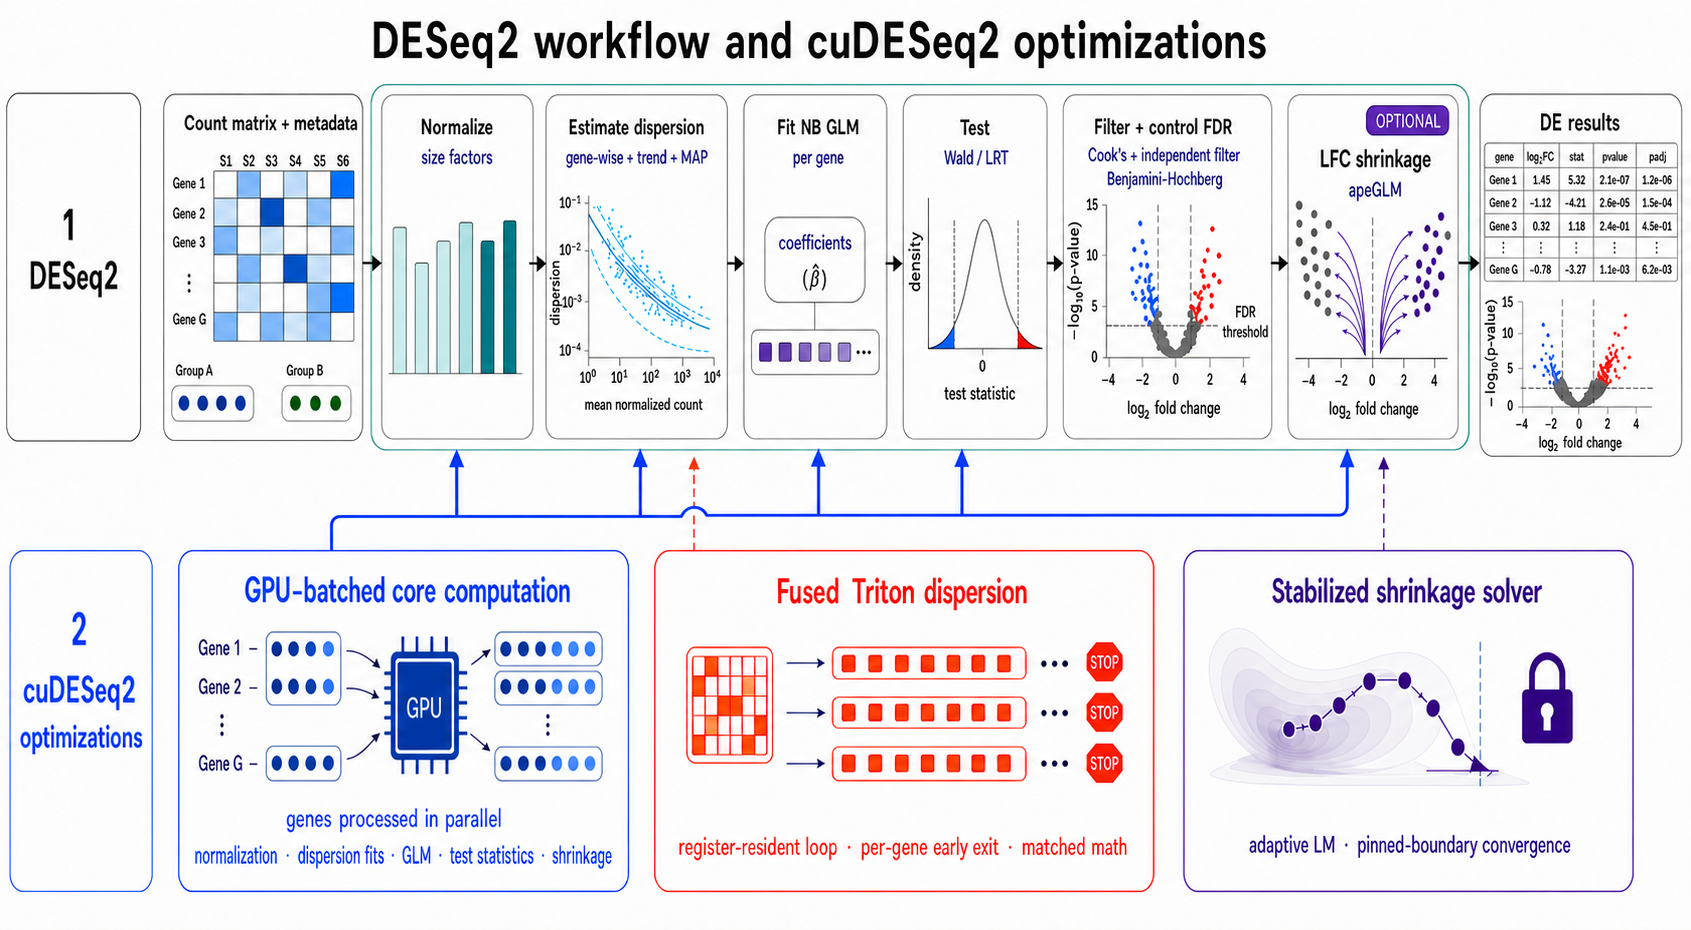
\includegraphics[width=\linewidth]{figures/gpt_schematic.png}
\caption{Overview of \cudeseq. DESeq2's per-gene, sequential CPU work
(dispersion estimation, the negative-binomial GLM, and apeGLM LFC shrinkage) is
batched across all genes on the GPU. The launch-bound dispersion loop runs in one
of three execution modes (eager, CUDA-graph chunked replay, or a fused Triton
kernel), and every stage is validated against R~DESeq2 to floating-point
precision.}
\label{fig:schematic}
\end{figure}

A bottleneck of this shape, many independent fits of identical form, suits a GPU
well. The established route to a faster DESeq2 has nonetheless been algorithmic
and CPU-bound. glmGamPoi \citep{ahlmanneltze2020glmgampoi} fits the
Gamma--Poisson GLM $6$--$13\times$ faster than DESeq2 and edgeR with sub-linear
scaling in cells, and DESeq2 can delegate its dispersion and GLM fits to it.
PyDESeq2 \citep{muzellec2023pydeseq2}, a Python reimplementation, improves
interoperability with the modern data-science stack and speed on large datasets,
though by its authors' own account it yields results that are ``similar, but not
identical'' to DESeq2; it too runs on the CPU and parallelizes across cores. GPU
acceleration has meanwhile transformed adjacent single-cell workflows, where
rapids-singlecell and ScaleSC report $15$--$20\times$ end-to-end speedups
\citep{hu2025scalesc}, but those gains come from the dense and sparse
linear-algebra core: PCA, neighbor graphs, clustering. The per-gene
negative-binomial inference where bulk DE spends its time is left untouched. To
our knowledge, DESeq2's dispersion--GLM--shrinkage path has no GPU
implementation.

Fidelity is the hard part. Whatever substitutes for the reference also
substitutes for its gene calls, effect sizes and FDR estimates, and reproducing
those exactly is difficult: DESeq2's behavior is fixed by a long list of clamps,
priors and line searches, and by a seeded Monte-Carlo estimator. Numerical GPU
ports of CPU code routinely diverge from their references, a hazard reported in
single-cell GPU work, which had to reconcile GPU/CPU discrepancies explicitly
\citep{hu2025scalesc}. Speedups built on approximation or resampling give up the
fidelity that makes the output substitutable in the first place.

We present \cudeseq, a from-scratch PyTorch \citep{paszke2019pytorch}
reimplementation of the DESeq2 pipeline that batches the per-gene work across
genes on the GPU while reproducing R~DESeq2~1.30.1 to floating-point precision at
\emph{every} intermediate quantity, not only the final call. Our effort went
where the cost is: the launch-bound dispersion loop, for which we provide three
interchangeable execution modes (eager, a CUDA-graph chunked replay
\citep{nvidia2024cudagraphs}, and a fully fused Triton kernel
\citep{tillet2019triton}), and the apeGLM shrinkage optimizer, which we port to
run batched on the GPU while reproducing the reference's optimum on a posterior
that is bimodal for the extreme-effect genes.

\noindent\textbf{Contributions.}
\begin{enumerate}[leftmargin=1.6em,label=(\roman*)]
  \item A batched GPU port of DESeq2's \texttt{fitDisp} (Cox--Reid gradient
        ascent), operation-for-operation faithful to the reference and validated
        against R at every intermediate quantity.
  \item A CUDA-graph mode (chunked replay) that removes launch overhead from the
        dispersion loops, using a capture-safe no-pivot LU in place of cuSOLVER.
  \item A fully fused Triton kernel: one program per gene runs the whole
        gradient-ascent loop in registers with per-gene early exit.
  \item A batched, on-device port of apeGLM's own L-BFGS optimizer (limited-memory
        BFGS with a strong-Wolfe line search). Because the shrinkage posterior is
        bimodal for extreme-effect genes, the shrunk value is the local optimum the
        reference's solver reaches from its initialization; porting that exact
        optimizer---rather than a batched Newton, which would settle in a different
        basin---reproduces R's shrunk log-fold-changes and keeps the whole
        pipeline on the GPU with no serial per-gene fallback.
  \item A per-step, reproducible benchmark methodology against single- and
        multi-core R, with an empirical roofline analysis.
\end{enumerate}

% ===========================================================================
\section{Methods}

\subsection{The DESeq2 pipeline and its cost profile}
\label{sec:pipeline}
DESeq2 \citep{love2014deseq2} models each gene independently with a
negative-binomial GLM. For gene $g$ with counts $K_{gi}$ over samples
$i=1,\dots,S$, design matrix $X\in\mathbb{R}^{S\times P}$, and size factors
$s_i$, it assumes $K_{gi}\sim\mathrm{NB}(\mu_{gi},\alpha_g)$ with
$\mu_{gi}=s_i\exp(x_i^{\!\top}\beta_g)$ and variance
$\mu_{gi}+\alpha_g\mu_{gi}^2$, and runs five stages:
\begin{enumerate}[leftmargin=1.6em]
  \item \textbf{Normalization}: median-of-ratios size factors.
  \item \textbf{Dispersion estimation}: gene-wise Cox--Reid MLE, a parametric
        mean--dispersion trend, empirical-Bayes MAP shrinkage, and an outlier
        rule. This is the dominant cost.
  \item \textbf{GLM fit / testing}: IRLS negative-binomial GLM, Wald / LRT.
  \item \textbf{Significance}: Cook's-distance filter, independent filtering,
        Benjamini--Hochberg adjustment.
  \item \textbf{LFC shrinkage}: apeGLM \citep{zhu2019apeglm}, a Cauchy-prior
        MAP estimate of the effect size.
\end{enumerate}
Stages 2, 3 and 5 are per-gene iterative optimizations executed sequentially in
R's C++ core, and each is embarrassingly parallel across genes.
Dispersion estimation dominates the wall time
(Sec.~\ref{sec:realtiming}), because its gene-wise MLE maximizes the Cox--Reid
adjusted profile log-likelihood
\begin{equation}
\ell_{\mathrm{CR}}(\alpha_g)=\sum_{i=1}^{S}\log \mathrm{NB}\!\bigl(K_{gi};\mu_{gi},\alpha_g\bigr)
\;-\;\tfrac12\log\det\!\bigl(X^{\!\top} W_g X\bigr),
\label{eq:cr}
\end{equation}
with $W_g=\operatorname{diag}\!\bigl(\mu_{gi}/(1+\alpha_g\mu_{gi})\bigr)$; the
$\log\det$ Cox--Reid adjustment couples every sample and must be recomputed each
iteration.

\subsection{A parity-first batched port}
\label{sec:port}
Our design rule is to reproduce the reference algorithm operation-for-operation
instead of re-deriving it, using the same optimizer, line search, clamps and
constants in IEEE double precision (fp64) throughout, so that every intermediate
quantity matches R
(Sec.~\ref{sec:parity-method}). Concretely, each per-gene loop in R becomes a
tensor program over all $G$ genes at once: the per-gene solver state
($\log\alpha_g$, $\beta_g$, step sizes, convergence flags) is carried as
$(G,\cdot)$ tensors, and a gene that has converged is frozen as a masked no-op so
the batch runs to the slowest gene's iteration count.

Three of the five stages batch directly and need no special machinery.
\emph{Normalization} computes median-of-ratios size factors, using a $0.5$
quantile (rather than a median primitive) so that even-sample-count averaging
matches R exactly, with a positive-counts geometric-mean fallback when every gene
has at least one zero. The \emph{GLM fit} is a batched IRLS negative-binomial
solve: working weights $W=\mu/(1+\alpha\mu)$, working response
$z=\log(\mu/s)+(K-\mu)/\mu$, and normal equations
$(X^{\!\top}WX+\lambda I)\beta=X^{\!\top}Wz$ solved for all genes in one batched
factorization (ridge $\lambda=10^{-6}$, deviance-ratio convergence
$<\!10^{-8}$, $\le250$ iterations), returning $\beta$, $\mu$ and the hat-matrix
diagonals; Wald standard errors follow from the sandwich form
$\mathrm{SE}=\sqrt{c^{\!\top}(M{+}\lambda)^{-1}M(M{+}\lambda)^{-1}c}$ and the LRT
from the full/reduced deviance difference. \emph{Significance} (Cook's-distance
outlier removal, independent filtering, BH) involves no per-gene optimizer at
all: Cook's distances and the BH adjustment are closed-form, and independent
filtering sweeps candidate cutoffs with the rejection curve smoothed by a robust
LOWESS. With nothing per-gene to batch, that stage stays on the host in
NumPy/SciPy. The remaining engineering effort goes to the two iterative
optimizers described below, the dispersion fit and apeGLM.

\subsection{Batched dispersion estimation}
\label{sec:disp}
The dispersion stage is a faithful batched port of DESeq2's \texttt{fitDisp} and
has three parts. \textbf{(i) Gene-wise Cox--Reid MLE.} We maximize
Eq.~\ref{eq:cr} over $a=\log\alpha$ by gradient ascent with Armijo
backtracking. Each iteration proposes $a'=a+\kappa\,\partial_a\ell_{\mathrm{CR}}$
clipped to $[-30,10]$, accepts it when the Armijo condition holds
($\varepsilon=10^{-4}$), and adapts the step: on acceptance
$\kappa\leftarrow\min(1.1\kappa,\kappa_0)$ with a halving every fifth acceptance,
on rejection $\kappa\leftarrow\kappa/2$; it stops when
$\Delta\ell_{\mathrm{CR}}<10^{-6}$ or $a$ drops below a floor, to a cap of $100$
iterations. Two R-matching safeguards follow the loop: a \emph{noIncrease revert}
that restores the initial estimate if the objective failed to improve, and a
deterministic $100$-point coarse/fine \emph{grid fallback} for genes R would flag
as non-converged. \textbf{(ii) Parametric trend.} We fit
$\alpha\approx a_0+a_1/\bar\mu$ by iteratively reweighting a Gamma-family,
identity-link GLM over the genes with $\mathrm{dispGeneEst}>100\cdot\mathrm{minDisp}$,
converging on $\sum\log(\text{coef}/\text{coef}_{\text{old}})^2<10^{-6}$, with a
trimmed-mean trend as fallback. \textbf{(iii) MAP shrinkage.} A log-normal prior
centered on the trend shrinks the gene-wise estimates; its variance comes from
the MAD of log-residuals, in closed form
$\max\!\bigl(s^2-\psi_1(\tfrac{m-p}{2}),\,0.25\bigr)$ at ample residual degrees of
freedom and from a stochastic KL-divergence grid search when
$m-p\le3$. The MAP re-runs the same gradient ascent with the prior term enabled
and, matching R, with the revert and grid fallback disabled; an outlier
rule keeps the raw MLE when $\log\alpha_{\text{MLE}}$ exceeds the trend by more
than $2s$.

The KL-divergence branch is the one place we cannot be bit-identical to R: it
mirrors R's \texttt{set.seed(2)} Monte-Carlo estimator, and NumPy's
Mersenne-Twister stream differs from R's. The resulting discrepancy is confined
to a few small-dof genes and is differential-expression-equivalent
(Sec.~\ref{sec:parity}); every other quantity in this stage is reproduced to
floating-point tolerance.

\subsection{Three execution modes for the dispersion loop}
\label{sec:modes}
The gradient-ascent loop is where the launch-bound overhead concentrates
(Sec.~\ref{sec:realtiming}); it is therefore the only stage with alternative
execution backends, and every other stage runs the eager code in all modes.
The three modes compute identical mathematics and differ only in how the loop is
dispatched (Table~\ref{tab:modes}); they are selected per call
(\texttt{fit\_dispersions(..., use\_cuda\_graph, use\_triton)}) or via the
\texttt{GPU\_DESEQ\_ACCEL} environment variable.

\begin{table}[htbp]\centering
\caption{The three execution modes for the dispersion loop.}
\label{tab:modes}
{\footnotesize
\begin{tabular}{llll}
\toprule
Mode & Dispatch & Fidelity & Designs \\\midrule
eager  & one kernel per tensor op        & reference          & any $P$ \\
graph  & replay a captured CUDA graph     & bit-identical to eager & any $P$ \\
Triton & one fused kernel per gene        & $\sim$1e-14 vs R    & $P\in\{2,\dots,6\}$ \\\bottomrule
\end{tabular}}
\\[3pt]
{\footnotesize Triton and graph fall back to eager for unsupported designs or on
CPU.}
\end{table}

\subsection{CUDA-graph chunked replay}
\label{sec:graph}
In eager mode each gradient-ascent iteration launches a handful of tiny kernels
over $1$--$10$\,MB arrays, so the loop is dominated by launch latency
(Sec.~\ref{sec:roofline}). Capturing the loop as a CUDA graph amortizes that cost
to a single replay, but two obstacles must be cleared. First, \emph{early exit}:
a fixed full-length capture would force every gene to the maximum iteration count,
which wastes the typical $15$--$40$-iteration case. We instead capture a
$K{=}10$-iteration graph over persistent state buffers and replay it in a loop
with a convergence check between chunks. A chunk always runs to its boundary, so
a gene that converges mid-chunk executes further iterations; those are exact
no-ops, because a converged gene is frozen by the same mask the eager loop uses,
and $K$ divides the iteration cap so the budget is never exceeded. The replayed
result is therefore \emph{bit-identical to eager} --- which also requires the two
paths to share operand types, not just arithmetic: passing the prior variance to
the eager loop as a Python scalar rather than the same $0$-dim tensor the graph
buffers lowers division to a reciprocal-multiply and costs one ulp per iteration.
Second, \emph{cuSOLVER}: the Cox--Reid term needs $\log\det(b)$ and
$\operatorname{tr}(b^{-1}\,\mathrm{d}b)$ with $b=X^{\!\top}WX$, and
\texttt{slogdet}/\texttt{solve} host-synchronize and cannot be captured. Since
$b$ is symmetric positive-definite for full-rank $X$, we replace them with an
unrolled \emph{no-pivot LU} (\texttt{\_logdet\_and\_tr\_binv\_db}) that returns
both quantities and matches the \texttt{linalg} path to $\sim$1e-15 for
$P=2\dots6$. Captured graphs are cached by
$(G,S,P,K,\text{prior},\text{dtype},\text{device})$; the prior variance is passed
as a scalar tensor so one graph serves datasets with different priors.

\subsection{Triton full-loop fusion}
\label{sec:triton}

\begin{figure}[htbp]\centering
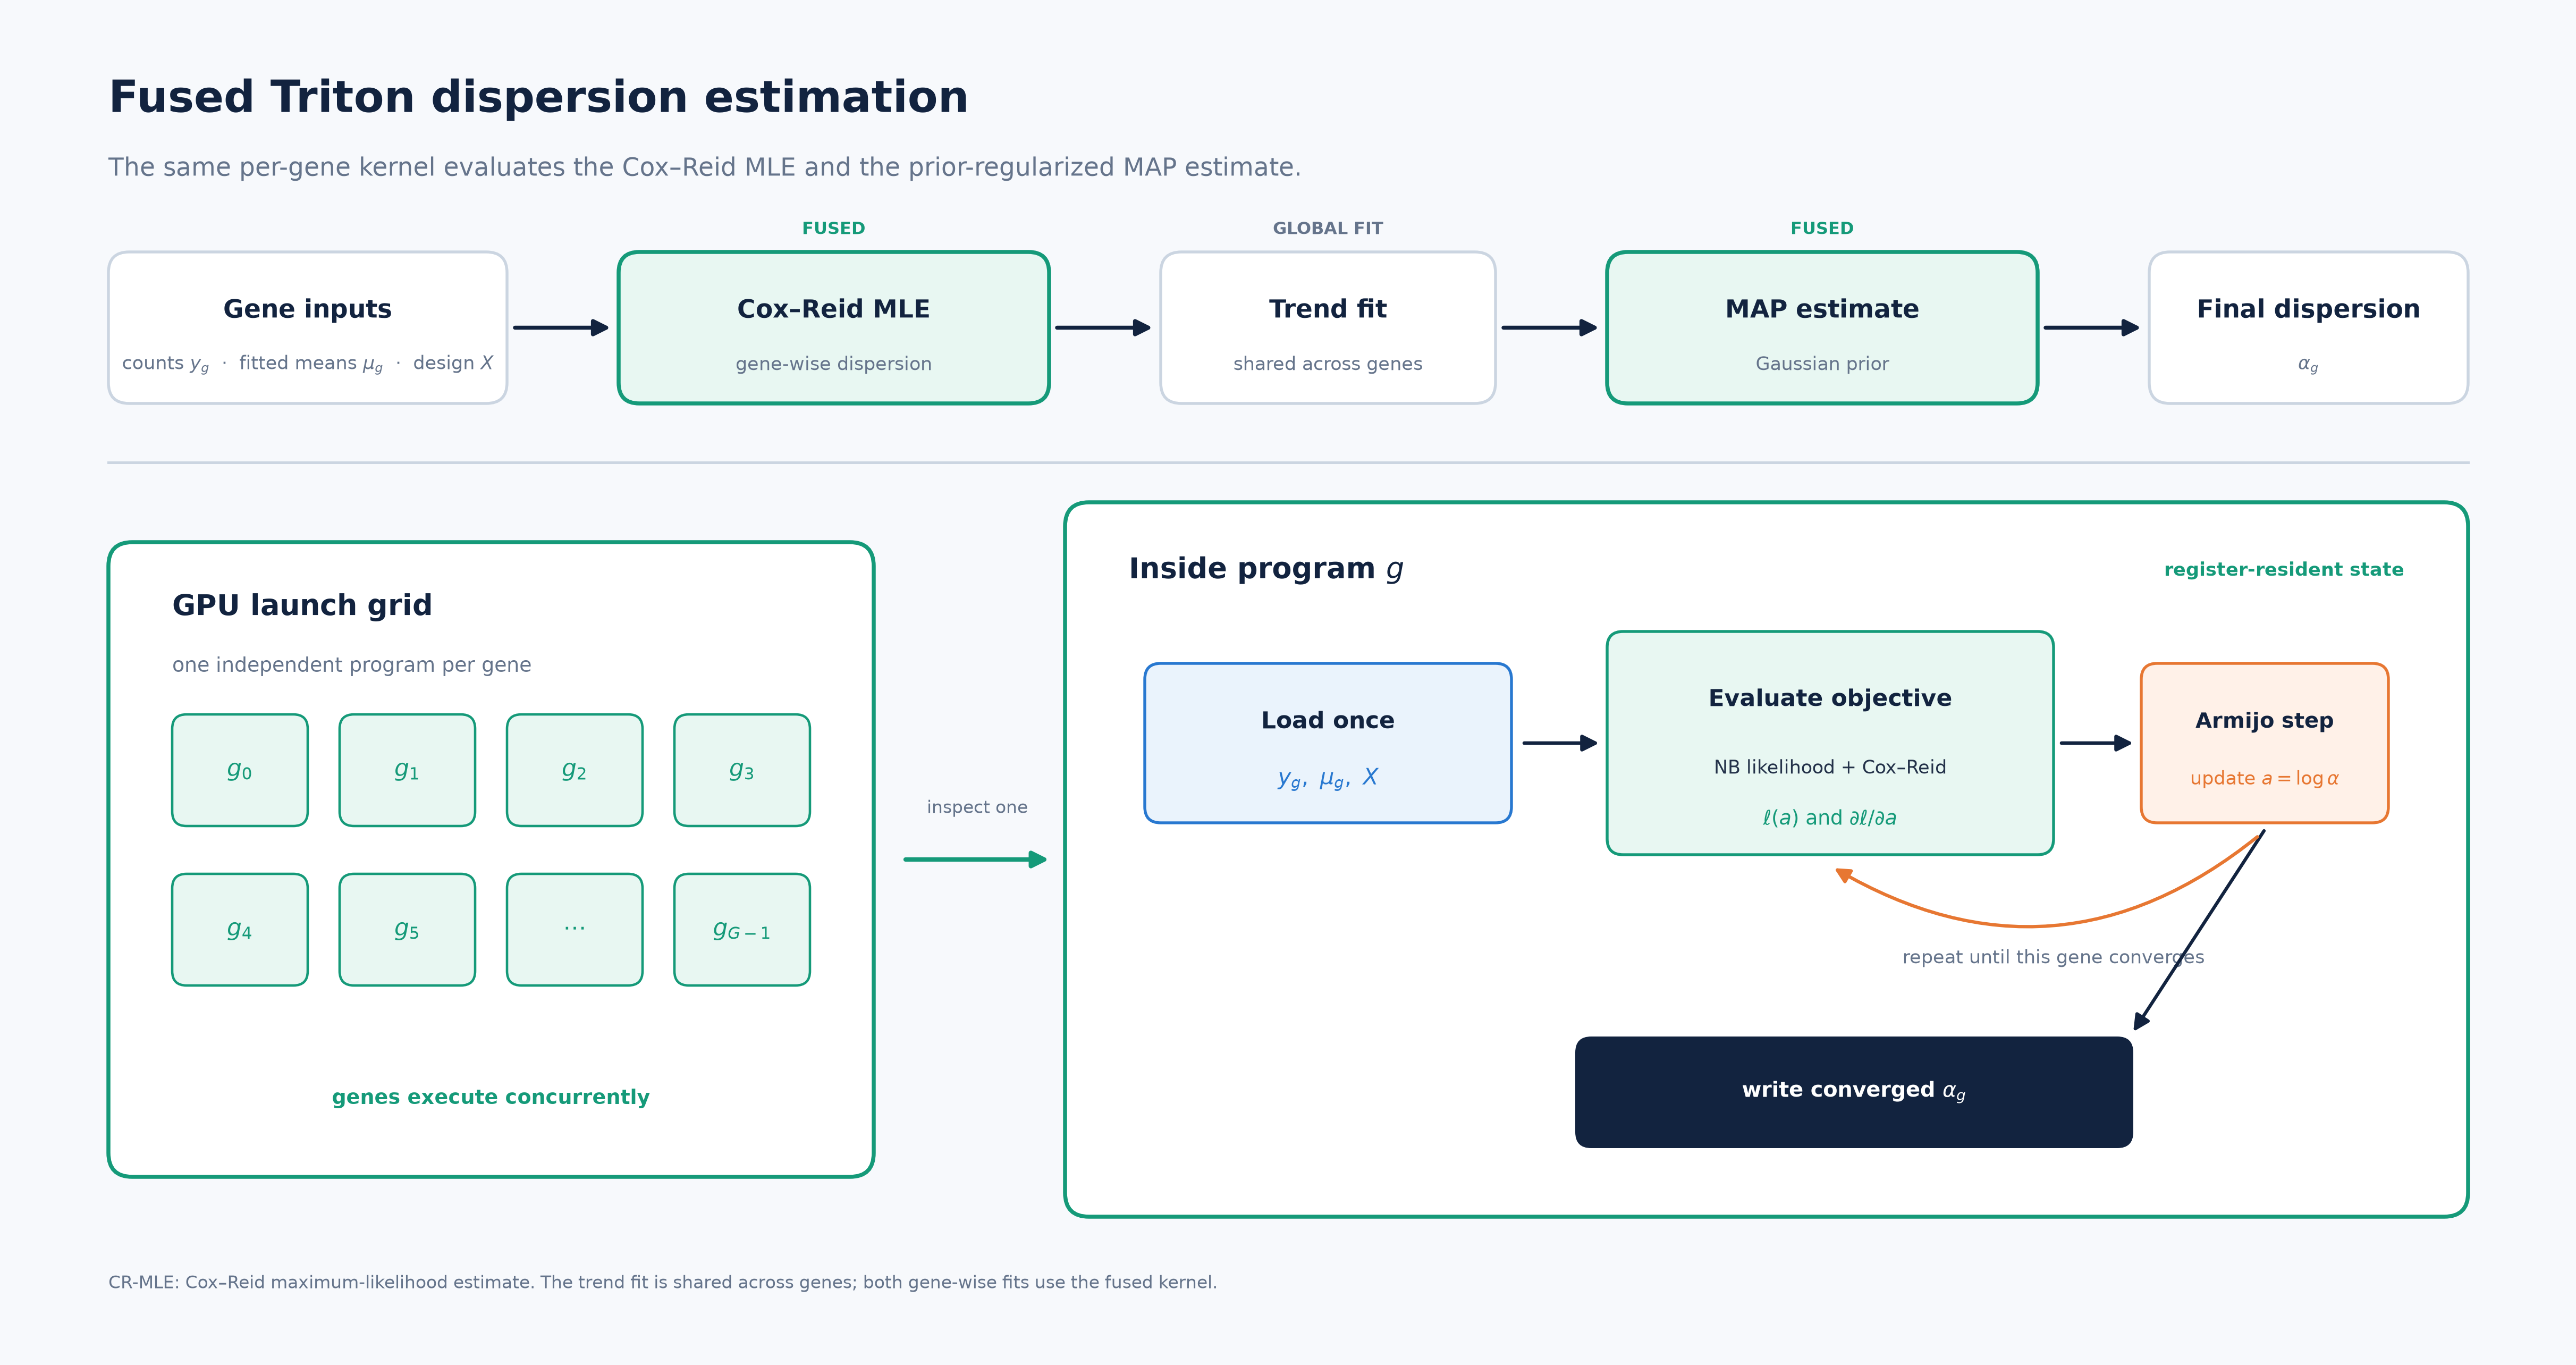
\includegraphics[width=\linewidth]{figures/triton_dispersion_schematic.png}
\caption{The fused Triton dispersion kernel. One kernel handles both gene-wise
fits of the dispersion pipeline: the Cox--Reid MLE, and the MAP shrinkage with a
Gaussian prior that follows the trend fit (the trend fit itself runs outside
Triton). One Triton program is launched per gene; it loads $\mathbf{y}_g$,
$\boldsymbol{\mu}_g$ and the design $\mathbf{X}$ once, then runs every iteration
of the gradient ascent register-resident, with the NB log-likelihood, the
Cox--Reid term $-\tfrac12\log\det\mathbf{B}$ ($\mathbf{B}=\mathbf{X}^{\!\top}
\mathbf{W}\mathbf{X}$), the $\log\alpha$-gradient and the Armijo line search all
fused into the loop body. Only the converged $a_g=\log\alpha_g$ is written back
to global memory. Supplementary
Algorithms~\ref{alg:triton-overview}--\ref{alg:triton-detail} give the
pseudocode.}
\label{fig:triton}
\end{figure}

The Triton mode fuses the entire per-gene fit into one program (one per gene;
Fig.~\ref{fig:triton}).
Its counts, $\mu$ and design columns are loaded once into registers, and the whole
gradient ascent then runs register-resident: the Cox--Reid $P\times P$ solve
(closed-form $2\times2$ for $P{=}2$, an unrolled no-pivot LU for $P=3\dots6$), the NB
log-likelihood and $\log\alpha$-gradient (\texttt{lgamma}/\texttt{log1p} from
\texttt{libdevice}, \texttt{digamma} hand-implemented to match ATen's
\texttt{calc\_digamma} via a recurrence to $x\ge10$ followed by the Bernoulli
asymptotic series), and the Armijo line search. A per-gene \texttt{while} loop
lets each gene exit as soon as it converges, so the kernel does not run every
gene to the batch maximum. The kernel
is fp64 and covers $P\in\{2,\dots,6\}$ (falling back to eager otherwise); it matches R
to $\sim$1e-14 but is \emph{not} bit-identical to eager, because the fused
reduction order differs. Non-converged or high-dispersion genes receive the same
noIncrease and grid fallback as the eager path.

Covering a range of $P$ takes one more step than it appears to. The eager path
writes the $P\times P$ elimination as a Python loop over tensor slices, but
Triton's frontend admits no local arrays and no compile-time sequence building,
so a register-resident matrix cannot be indexed by a loop variable: the algebra
has to appear as straight-line code specialized to each $P$. Because that grows
quadratically---$174$ lines at $P{=}6$ against $20$ at $P{=}2$---we emit it from
a generator that mirrors the eager elimination operation for operation, rather
than hand-writing each case. Only the $P\in\{2,4\}$ arms remain hand-written.
Generated and hand-written arms are checked against the eager Cox--Reid term at
fixed $\alpha$, which isolates the linear algebra from the optimizer's path: the
log-posterior agrees to $5$e-16 and its gradient to ${\sim}3$e-14 for every
covered $P$. Designs outside the covered range raise rather than silently fit a
truncated model, since the kernel reads a fixed number of design columns.

\subsection{Batched port of the apeGLM optimizer}
\label{sec:apeglm}
apeGLM \citep{zhu2019apeglm} shrinks the log-fold-change by maximizing a per-gene
posterior: the NB likelihood times a heavy-tailed Cauchy prior on the coefficient
of interest (prior scale set by empirical Bayes,
$\tau=\min(\sqrt{\widehat{\text{var}}},1)$) and a wide Gaussian on the nuisance
coefficients. Reproducing its output faithfully turns on a subtlety of this
objective: for extreme-effect, low-count genes it is \emph{bimodal} in the shrunk
coefficient---a sharp likelihood mode far from zero and a prior mode near
zero---and the two can be nearly tied in posterior mass. The value the reference
reports is therefore not simply ``the'' MAP but the particular local optimum its
solver reaches from its initialization. In DESeq2, \texttt{lfcShrink} runs apeGLM
with \texttt{method="nbinomCR"}, whose estimate comes from a limited-memory BFGS
solver (LBFGS++ via \texttt{RcppNumerical}) started at a fixed
$\pm0.1$-alternating point. A batched Newton method, by contrast, would locate the
\emph{global} optimum and so disagree with R on exactly these genes---a
difference we confirmed is not our solver ``failing'' but landing in the other,
equally-valid basin.

We therefore port the reference's optimizer itself, vectorized across genes on the
GPU: limited-memory BFGS ($m{=}6$) with a backtracking strong-Wolfe line search
($\mathrm{ftol}=10^{-4}$, $\mathrm{wolfe}=0.9$, dec$=0.5$, inc$=2.1$), the
two-loop recursion, an initial step $1/\lVert d\rVert$ reset to $1$ each
iteration, and apeGLM's gradient-norm and objective-change stopping tests---all
from the identical $\pm0.1$ initialization. Running the same algorithm from the
same start makes the same basin selection, so the batched solve reproduces R's
shrunk log-fold-changes (Sec.~\ref{sec:parity}) rather than a different optimum.
The per-gene solver state ($\beta_g$, the $m$-step history, step size, convergence
flags) is carried as $(G,\cdot)$ tensors exactly as in the dispersion loop, so the
whole shrinkage stage runs batched on the GPU with no serial per-gene fallback.
The reported \texttt{lfcSE} is the square root of the shrunk coefficient's
diagonal of the inverse observed information at the optimum.

\subsection{Parity methodology}
\label{sec:parity-method}
Reference fixtures are generated by \texttt{generate\_r\_fixtures.R} against
R~DESeq2~1.30.1, and every intermediate is checked against R: size factors,
\texttt{dispGeneEst}, \texttt{dispFit}, \texttt{dispMAP}, $\beta$, $\mu$, the
hat-matrix diagonals, Cook's distances, Wald SE, the LRT statistic, and the
apeGLM shrunk LFC/SE. Errors are reported as p95 relative values, or absolute
values where a quantity crosses zero, on designs of rank $P=2$ and $P=4$.
Tolerances and the measured
per-substep results, including the real-data end-to-end comparison, are reported
in Sec.~\ref{sec:parity}.

% ===========================================================================
\section{Results}

\subsection{Experimental setup}
\note{Provenance: A100-SXM4-40GB, torch 2.6/CUDA 12.4, R~DESeq2~1.30.1 on a
12-core host, median-of-N, warm timings, CUDA-synced. R runs single-threaded
everywhere except the explicit ``R 12-core'' column of
Table~\ref{tab:perstep}, which uses \texttt{DESeq(parallel=TRUE)} with a
\texttt{MulticoreParam(12)}. Reproducible harnesses: real-data
parity and timing in bench/ (\texttt{bench/bench.py}), synthetic scaling in
benchmarks/.}
\todo{\textbf{GAP:} add a second GPU (L4) and a larger-core R box (32--64).}
We validate on three real RNA-seq datasets sliced into six designs spanning
$P=2$--$5$ model terms: pasilla (\emph{Drosophila}, $n{=}7$, one- and two-factor),
airway (human, $n{=}8$, three design slices), and a 300-sample GTEx whole-blood
vs.\ muscle contrast ($54{,}922$ genes). Scaling studies use fixed-seed
negative-binomial simulations where the gene and sample axes can be swept
independently.

\subsection{Numerical parity with R}
\label{sec:parity}
Correctness is checked per substep against R on all six real datasets, each
against an explicit PASS tolerance (Table~\ref{tab:parity}). A separate synthetic
step-parity suite (\texttt{tests/test\_r\_step\_parity.py}, 76/76) confirms the
same agreement at controlled sizes, and more tightly: size factors agree to
$<$1e-10, gene-wise dispersion to $\sim$1e-9, and MAP dispersion, $\beta$, $\mu$,
the Hessian and Wald SEs to $\sim$1e-6 relative. A further suite
(\texttt{tests/test\_triton\_dispersion.py}) pins the fused kernel against the
eager path once per covered $P$, the axis along which its specialized arms
(Sec.~\ref{sec:triton}) could diverge without any other test noticing.

\begin{table}[htbp]\centering
\caption{Per-substep agreement with R~DESeq2~1.30.1 across all six real datasets.
Each substep is scored by its natural metric against a fixed PASS tolerance;
``worst'' is the least-favorable of the six datasets. \fact{Reproduce:
\texttt{bench/bench.py} $\to$ \texttt{bench/results/parity.json}.}}
\label{tab:parity}
\begin{tabular}{lllr l}
\toprule
Substep & Metric & PASS tol & Worst obs. & Result \\\midrule
normalization & max rel.\ $\Delta$ & $\le$1e-6 & 5.7e-15 & 6/6 pass \\
dispersion & p95 rel.\ $\Delta$ & $\le$0.10 & 0.067 & 6/6 pass \\
glm\_fit & p95 $|\Delta|$ (LFC) & $\le$1e-2 & 4.8e-3 & 6/6 pass \\
significance & Jaccard@0.05 & $\ge$0.95 & 0.971 & 6/6 pass \\
lfc\_shrink & Pearson $r$ & $\ge$0.90 & 0.997 & 6/6 pass \\\bottomrule
\end{tabular}
\end{table}

All 30 substep checks pass, and five of the six dispersions land within 0.4\%.
The one loose case is a non-issue for differential expression: \texttt{airway}
dispersion reaches 6.7\% because at $n{=}8$, $P{=}5$ (dof~3) R's
\texttt{set.seed(2)} Mersenne-Twister in the small-dof prior-variance estimator is
not reproducible in NumPy, and 6.7\% is DE-equivalent. The apeGLM shrinkage
matches R to Pearson $r\ge0.997$ on every dataset; its only residual is a handful
of flat, near-degenerate genes (0 on three datasets, at most 12 of 33{,}469 on
\texttt{airway\_cell}) where two limited-memory-BFGS implementations break a tie
between equal-posterior optima differently, with p95 $|\Delta|\le$4e-4 and no
effect on any call. Across modes, the graph path is bit-identical to eager on
every substep of all six datasets (max $|\Delta|=0$ exactly, and each mode is
reproducible run to run). Triton is deliberately not: its fused reduction order
and hand-written \texttt{digamma} move the last bits, so across all six designs
---every one of which it now covers---it agrees with eager to $\sim$1e-7 in
dispersion on the five small-$n$ sets, widening to a worst case of $2.6$e-1
relative on one \texttt{gtex} gene and $5.7$e-3 absolute in the shrunk LFC. Those
genes sit at the dispersion-grid boundary or on the flat posterior optima
described above; no PASS verdict and no DE call changes.

\subsection{Real-data timing versus R}
\label{sec:realtiming}
\begin{table}[htbp]\centering
\caption{End-to-end wall time on the six real datasets: single-threaded
R~DESeq2~1.30.1 vs.\ cuDESeq2's three modes on a single A100. Speedup is the best cuDESeq2
mode vs.\ R. \fact{Reproduce: \texttt{bench/bench.py} $\to$
\texttt{bench/results/timings.json}.}}
\label{tab:realtiming}
\begin{tabular}{lrrrrrr}
\toprule
Dataset & $P$ & $n$ & R (s) & eager & graph & Triton \\
        &     &     &       & (ms)  & (ms)  & (ms)   \\\midrule
pasilla       & 2 &   7 &   9.3 & 1137 &  784 &  689 \\
pasilla\_2fac & 3 &   7 &  10.3 & 1510 &  941 &  866 \\
airway\_dex   & 2 &   8 &  25.7 & 1684 & 1374 & 1339 \\
airway\_cell  & 4 &   8 &  27.9 & 4181 & 3573 & 3459 \\
airway        & 5 &   8 &  33.5 & 2324 & 1610 & 1507 \\
gtex          & 2 & 300 & 350.4 & 8422 & 8537 & 4582 \\\bottomrule
\end{tabular}
\\[3pt]
{\footnotesize Best-mode speedup vs.\ R: pasilla 13.5$\times$, pasilla\_2fac
11.9$\times$, airway\_dex 19.2$\times$, airway\_cell 8.1$\times$, airway
22.2$\times$, gtex 76.5$\times$. Triton is the best mode on all six.}
\end{table}

The graph and Triton flags accelerate \emph{only} the dispersion substep; the
other four substeps---including the apeGLM shrink, which now also runs batched on
the GPU---execute identical code in every mode. Those rows of
Table~\ref{tab:realsubstep} are accordingly equal for eager and graph up to
measurement noise, since the two feed them bit-identical dispersions. Triton is
the exception: the shrinkage optimizer iterates to a tolerance, so the last-bit
differences in its dispersions shift its iteration count, and on \texttt{gtex}
that makes \texttt{lfc\_shrink} materially faster rather than equal. End-to-end
speedup is
therefore set by whichever cuDESeq2 substep is slowest relative to R. On the large
\texttt{gtex} set that is dispersion, which Triton cuts from 231\,s to 0.2\,s,
driving the highest end-to-end speedup, 76.5$\times$. On the small-$n$ sets the
apeGLM shrink is the heaviest per-gene stage---its limited-memory-BFGS iterations
on the bimodal extreme-effect genes dominate---which is what caps
\texttt{airway\_cell} at 8$\times$. Triton is now the fastest mode on all six
designs. It was not always: the multi-factor cases \texttt{airway} ($P{=}5$) and
\texttt{pasilla\_2fac} ($P{=}3$) previously fell outside the kernel's $P\in\{2,4\}$
coverage and dispatched silently to the eager loop, so their Triton and eager
dispersion times were identical to within noise. Extending the Cox--Reid solve to
$P\in\{2,\dots,6\}$ (Sec.~\ref{sec:triton}) cuts their dispersion substep by
$4.0\times$ and $8.9\times$ against the eager loop they used to fall back to
(1203$\to$304\,ms and 730$\to$82\,ms, same run),
which is what moves both datasets' best mode from graph to Triton. Fusion never
lost on these designs; it simply had not been written for them.
All three modes are shipped because the best choice still depends on the design
and the sample count.

\begin{table}[htbp]\centering
\caption{Per-substep wall time (ms) on the real datasets, single-threaded R vs.\
the three cuDESeq2 modes. Graph/Triton differ from eager only in \texttt{dispersion}; all
other rows are eager code and equal across modes up to measurement noise.
\fact{Reproduce: \texttt{bench/bench.py} $\to$ \texttt{bench/results/TABLES.md}.}}
\label{tab:realsubstep}
{\footnotesize
\begin{tabular}{llrrrr}
\toprule
Dataset & Substep & R & eager & graph & Triton \\\midrule
pasilla & dispersion & 2335 & 415 & 71 & 21 \\
        & glm\_fit & 2138 & 36 & 36 & 36 \\
        & significance & 277 & 62 & 61 & 62 \\
        & lfc\_shrink & 4382 & 623 & 616 & 570 \\
        & \textbf{total} & \textbf{9307} & \textbf{1137} & \textbf{784} & \textbf{689} \\\midrule
pasilla\_2fac & dispersion & 2791 & 730 & 162 & 82 \\
        & glm\_fit & 1502 & 327 & 325 & 330 \\
        & significance & 240 & 59 & 60 & 59 \\
        & lfc\_shrink & 5637 & 393 & 392 & 394 \\
        & \textbf{total} & \textbf{10346} & \textbf{1510} & \textbf{941} & \textbf{866} \\\midrule
airway\_dex & dispersion & 6212 & 419 & 109 & 52 \\
        & glm\_fit & 5666 & 51 & 51 & 53 \\
        & significance & 1299 & 125 & 123 & 145 \\
        & lfc\_shrink & 12290 & 1087 & 1091 & 1089 \\
        & \textbf{total} & \textbf{25664} & \textbf{1684} & \textbf{1374} & \textbf{1339} \\\midrule
airway\_cell & dispersion & 5724 & 744 & 184 & 60 \\
        & glm\_fit & 4190 & 33 & 32 & 33 \\
        & significance & 362 & 117 & 116 & 118 \\
        & lfc\_shrink & 17423 & 3286 & 3240 & 3248 \\
        & \textbf{total} & \textbf{27899} & \textbf{4181} & \textbf{3573} & \textbf{3459} \\\midrule
airway & dispersion & 10423 & 1203 & 473 & 304 \\
        & glm\_fit & 4738 & 87 & 77 & 78 \\
        & significance & 365 & 120 & 120 & 120 \\
        & lfc\_shrink & 17717 & 912 & 939 & 1003 \\
        & \textbf{total} & \textbf{33456} & \textbf{2324} & \textbf{1610} & \textbf{1507} \\\midrule
gtex & dispersion & 231276 & 3501 & 3625 & 200 \\
        & glm\_fit & 42321 & 424 & 416 & 396 \\
        & significance & 17865 & 2765 & 2765 & 2750 \\
        & lfc\_shrink & 56020 & 1729 & 1727 & 1233 \\
        & \textbf{total} & \textbf{350435} & \textbf{8422} & \textbf{8537} & \textbf{4582} \\\bottomrule
\end{tabular}}
\\[3pt]
{\footnotesize \texttt{normalization} omitted ($\le$4\,ms cuDESeq2 on every set);
full table in \texttt{bench/results/TABLES.md}. All six datasets were timed in a
single session on an otherwise idle GPU; absolute values shift by
$10$--$25$\,\% between sessions (\texttt{airway}, timed first, pays warmup), so
compare modes within a row rather than across runs.}
\end{table}

\subsection{Scaling on synthetic data}
\label{sec:roofline}
\note{ncu counters blocked $\Rightarrow$ empirical roofline: sustainable BW
1258 GB/s, but the loop's 1--10 MB arrays reach only 3--44\% of it, and
\_lp\_and\_dlp takes the same time for 2k vs 20k genes $\Rightarrow$
launch/latency-bound, not memory- or compute-bound. This is what graphs/fusion
attack.}
\begin{table}[htbp]\centering
\caption{Per-step wall time (ms), $60\times20000$ genes, single A100 vs R~DESeq2
(12-core box). \fact{Reproduce: \texttt{benchmarks/bench\_per\_step.py}.}
\todo{These synthetic-scaling numbers predate the batched-LBFGS apeGLM port
(Sec.~\ref{sec:apeglm}); regenerate the \texttt{lfc\_shrink} and TOTAL rows (the
other steps are unaffected) before submission.}}
\label{tab:perstep}
\begin{tabular}{lrrrrr}
\toprule
Step & R 1-thr & R 12-core & eager & graph & Triton \\\midrule
normalization & 473 & 473 & 1.2 & 1.2 & 1.2 \\
dispersion & 13923 & 8397$^\dagger$ & 349 & 213 & 80 \\
glm\_fit & 5137 & (bundled) & 11 & 11 & 11 \\
significance & 284 & 285 & 145 & 145 & 145 \\
lfc\_shrink & 8470 & 3201 & 92 & 92 & 92 \\\midrule
\textbf{TOTAL} & \textbf{28287} & \textbf{12356} & \textbf{598} & \textbf{462} & \textbf{330} \\\bottomrule
\end{tabular}
\\[3pt]
{\footnotesize $^\dagger$DESeq2 parallelizes dispersion+GLM as one gene-chunked
bundle; the two rows share it. Totals give Triton-vs-best-R speedups of
19.3/28.9/37.5/26.6$\times$ across the four cases.}
\end{table}
\note{Gene axis (2k vs 20k) and sample axis (2v2 pilot to 2000 samples): the
accelerators help most in the launch-bound small-sample regime (at n=4--6 the
graph gains 7.3$\times$ on the NR loop over eager, Triton 40$\times$); at $>$1000
samples the loop becomes compute-bound.
Multi-core R only beats single-thread at $\geq$20k genes (fork overhead below
that).}

\subsection{Ablations}
\begin{itemize}[leftmargin=1.4em]
  \item Fixed-length vs chunked CUDA graph: on the full dispersion stage
        0.8--1.1$\times$ $\to$ 1.7--3.4$\times$ (isolated NR loop, up to
        5.5$\times$); a fixed capture must run all 100 iterations, which costs
        more than the launches it saves.
  \item Fixed-iteration vs per-gene early-exit Triton (fixes the 20k regression).
  \item apeGLM: batched Newton (global optimum, mismatches R on bimodal genes)
        vs.\ the ported L-BFGS (reference's local optimum; parity restored).
  \item \texttt{GRAPH\_CHUNK} sweep (chunk 10 near-optimal).
\end{itemize}

% ===========================================================================
\section{Discussion}
\todo{Reference-faithful GPU DE is feasible and fast; the wins come from treating
per-gene fits as batched GPU work and from removing launch overhead, not from
approximation. State current scope honestly and the path to closing it.}

\noindent\textbf{Limitations.}
\begin{itemize}[leftmargin=1.4em]
  \item Tested designs: single factor (up to four levels), additive
        multi-factor (up to P=5), continuous. Not yet: interaction designs,
        $n<6$.
  \item Not implemented: \texttt{replaceOutliers} refit, \texttt{lfcShrink}
        types \texttt{normal}/\texttt{ashr}, \texttt{glmGamPoi}, VST/rlog.
  \item Triton path: $P\in\{2,4\}$ only (falls back to eager otherwise); not
        bit-identical to eager ($\sim$1e-14 vs R).
  \item Benchmarks: single A100, 12-core R host; DESeq2 1.30.1 only.
\end{itemize}
\todo{Future: more designs (interactions, many-level factors), additional shrink
types, GPU-side independent filtering / trend fit, multi-GPU cohorts.}

% ===========================================================================
\section*{Funding}
\todo{Grant numbers, or ``This work received no specific grant \dots''}

\section*{Conflict of Interest}
none declared.

\section*{Data and software availability}
Source code, tests, and benchmark harnesses are available at
\url{https://github.com/synthesizebio/gpu_deseq}. \todo{license, archived
release DOI.} Reproduce with:
\begin{lstlisting}
# parity (all three modes)
GPU_DESEQ_ACCEL={eager|graph|triton} pytest tests/
# per-step vs R (1-thread + k-core)
python benchmarks/bench_per_step.py --ncores 12
# roofline
python benchmarks/roofline_empirical.py
\end{lstlisting}

% Scaffold has no \cite yet; \nocite{*} renders the starter refs so the
% bibliography is non-empty. Remove once real \citep/\citet commands are added.
\nocite{*}
\bibliographystyle{plainnat}
\bibliography{references}

% ===========================================================================
\clearpage
\section*{Supplementary figures}
\addcontentsline{toc}{section}{Supplementary figures}
\label{sec:supplementary}

Supplementary Algorithm~\ref{alg:triton-overview} gives a high-level view of the
fused Triton dispersion fit sketched in Fig.~\ref{fig:triton}; Supplementary
Algorithm~\ref{alg:triton-detail} gives the full kernel, including the Armijo
line search, the step-size adaptation, and the Cox--Reid objective/gradient
routine shared by the CR--MLE and MAP passes.

% High-level companion to triton_dispersion_algorithm.tex.
% Uses only packages already loaded by paper/main.tex.
% Insert with: % High-level companion to triton_dispersion_algorithm.tex.
% Uses only packages already loaded by paper/main.tex.
% Insert with: % High-level companion to triton_dispersion_algorithm.tex.
% Uses only packages already loaded by paper/main.tex.
% Insert with: \input{triton_dispersion_overview_algorithm}

\begingroup
\newcounter{tritonoverviewline}
\setcounter{tritonoverviewline}{0}
\newcommand{\tritonOverviewLine}[2][0em]{%
  \stepcounter{tritonoverviewline}%
  \noindent
  \makebox[2.1em][r]{\arabic{tritonoverviewline}:}%
  \hspace{0.7em}\hspace*{#1}%
  \begin{minipage}[t]{\dimexpr\linewidth-3.2em-#1\relax}%
    #2
  \end{minipage}\par
}

\begin{figure}[htbp]
\small
\noindent\rule{\linewidth}{0.8pt}\par
\vspace{2pt}
\noindent
\refstepcounter{supalg}\label{alg:triton-overview}%
\textbf{Supplementary Algorithm~\thesupalg}\quad
\textsc{Fused Triton dispersion fit} (high-level)
\par
\vspace{2pt}
\noindent\rule{\linewidth}{0.4pt}\par
\vspace{4pt}

\noindent
\textbf{Require:}\;
counts $\mathbf{Y}\in\mathbb{N}_0^{G\times S}$;
fitted means $\boldsymbol{\mu}\in\mathbb{R}_{+}^{G\times S}$;
design $\mathbf{X}\in\mathbb{R}^{S\times P}$;
initial dispersions $\boldsymbol{\alpha}^{(0)}$;
optional MAP prior.
\par
\noindent
\textbf{Ensure:}\;
optimized log dispersions $\mathbf{a}$ and iteration counts $\mathbf{c}$.
\par
\vspace{4pt}

\tritonOverviewLine{\textbf{Launch} one Triton program for every gene $g$ in parallel.}
\tritonOverviewLine[1.2em]{Load $\mathbf{y}_g$, $\boldsymbol{\mu}_g$, and
  $\mathbf{X}$ once into program-local state.}
\tritonOverviewLine[1.2em]{Initialize
  $a\leftarrow\operatorname{clip}(\log\alpha_g^{(0)},-30,10)$ and
  step size $\kappa\leftarrow\kappa_0$.}
\tritonOverviewLine[1.2em]{\textbf{repeat} inside the same fused program}
\tritonOverviewLine[2.4em]{Compute the negative-binomial log-likelihood and
  Cox--Reid adjustment.}
\tritonOverviewLine[2.4em]{If fitting MAP dispersion, add the Gaussian prior
  on $a=\log\alpha$.}
\tritonOverviewLine[2.4em]{Compute the gradient $q\leftarrow\partial\ell/\partial a$.}
\tritonOverviewLine[2.4em]{Propose the gradient-ascent step
  $\widetilde a\leftarrow a+\kappa q$.}
\tritonOverviewLine[2.4em]{Accept or reject $\widetilde a$ using the Armijo
  condition; adapt $\kappa$.}
\tritonOverviewLine[1.2em]{\textbf{until} converged or \textit{maxit} is reached.}
\tritonOverviewLine[1.2em]{Store the final $a_g$ and iteration count $c_g$ once
  in global memory.}

\vspace{3pt}
\noindent\rule{\linewidth}{0.8pt}
\end{figure}
\endgroup


\begingroup
\newcounter{tritonoverviewline}
\setcounter{tritonoverviewline}{0}
\newcommand{\tritonOverviewLine}[2][0em]{%
  \stepcounter{tritonoverviewline}%
  \noindent
  \makebox[2.1em][r]{\arabic{tritonoverviewline}:}%
  \hspace{0.7em}\hspace*{#1}%
  \begin{minipage}[t]{\dimexpr\linewidth-3.2em-#1\relax}%
    #2
  \end{minipage}\par
}

\begin{figure}[htbp]
\small
\noindent\rule{\linewidth}{0.8pt}\par
\vspace{2pt}
\noindent
\refstepcounter{supalg}\label{alg:triton-overview}%
\textbf{Supplementary Algorithm~\thesupalg}\quad
\textsc{Fused Triton dispersion fit} (high-level)
\par
\vspace{2pt}
\noindent\rule{\linewidth}{0.4pt}\par
\vspace{4pt}

\noindent
\textbf{Require:}\;
counts $\mathbf{Y}\in\mathbb{N}_0^{G\times S}$;
fitted means $\boldsymbol{\mu}\in\mathbb{R}_{+}^{G\times S}$;
design $\mathbf{X}\in\mathbb{R}^{S\times P}$;
initial dispersions $\boldsymbol{\alpha}^{(0)}$;
optional MAP prior.
\par
\noindent
\textbf{Ensure:}\;
optimized log dispersions $\mathbf{a}$ and iteration counts $\mathbf{c}$.
\par
\vspace{4pt}

\tritonOverviewLine{\textbf{Launch} one Triton program for every gene $g$ in parallel.}
\tritonOverviewLine[1.2em]{Load $\mathbf{y}_g$, $\boldsymbol{\mu}_g$, and
  $\mathbf{X}$ once into program-local state.}
\tritonOverviewLine[1.2em]{Initialize
  $a\leftarrow\operatorname{clip}(\log\alpha_g^{(0)},-30,10)$ and
  step size $\kappa\leftarrow\kappa_0$.}
\tritonOverviewLine[1.2em]{\textbf{repeat} inside the same fused program}
\tritonOverviewLine[2.4em]{Compute the negative-binomial log-likelihood and
  Cox--Reid adjustment.}
\tritonOverviewLine[2.4em]{If fitting MAP dispersion, add the Gaussian prior
  on $a=\log\alpha$.}
\tritonOverviewLine[2.4em]{Compute the gradient $q\leftarrow\partial\ell/\partial a$.}
\tritonOverviewLine[2.4em]{Propose the gradient-ascent step
  $\widetilde a\leftarrow a+\kappa q$.}
\tritonOverviewLine[2.4em]{Accept or reject $\widetilde a$ using the Armijo
  condition; adapt $\kappa$.}
\tritonOverviewLine[1.2em]{\textbf{until} converged or \textit{maxit} is reached.}
\tritonOverviewLine[1.2em]{Store the final $a_g$ and iteration count $c_g$ once
  in global memory.}

\vspace{3pt}
\noindent\rule{\linewidth}{0.8pt}
\end{figure}
\endgroup


\begingroup
\newcounter{tritonoverviewline}
\setcounter{tritonoverviewline}{0}
\newcommand{\tritonOverviewLine}[2][0em]{%
  \stepcounter{tritonoverviewline}%
  \noindent
  \makebox[2.1em][r]{\arabic{tritonoverviewline}:}%
  \hspace{0.7em}\hspace*{#1}%
  \begin{minipage}[t]{\dimexpr\linewidth-3.2em-#1\relax}%
    #2
  \end{minipage}\par
}

\begin{figure}[htbp]
\small
\noindent\rule{\linewidth}{0.8pt}\par
\vspace{2pt}
\noindent
\refstepcounter{supalg}\label{alg:triton-overview}%
\textbf{Supplementary Algorithm~\thesupalg}\quad
\textsc{Fused Triton dispersion fit} (high-level)
\par
\vspace{2pt}
\noindent\rule{\linewidth}{0.4pt}\par
\vspace{4pt}

\noindent
\textbf{Require:}\;
counts $\mathbf{Y}\in\mathbb{N}_0^{G\times S}$;
fitted means $\boldsymbol{\mu}\in\mathbb{R}_{+}^{G\times S}$;
design $\mathbf{X}\in\mathbb{R}^{S\times P}$;
initial dispersions $\boldsymbol{\alpha}^{(0)}$;
optional MAP prior.
\par
\noindent
\textbf{Ensure:}\;
optimized log dispersions $\mathbf{a}$ and iteration counts $\mathbf{c}$.
\par
\vspace{4pt}

\tritonOverviewLine{\textbf{Launch} one Triton program for every gene $g$ in parallel.}
\tritonOverviewLine[1.2em]{Load $\mathbf{y}_g$, $\boldsymbol{\mu}_g$, and
  $\mathbf{X}$ once into program-local state.}
\tritonOverviewLine[1.2em]{Initialize
  $a\leftarrow\operatorname{clip}(\log\alpha_g^{(0)},-30,10)$ and
  step size $\kappa\leftarrow\kappa_0$.}
\tritonOverviewLine[1.2em]{\textbf{repeat} inside the same fused program}
\tritonOverviewLine[2.4em]{Compute the negative-binomial log-likelihood and
  Cox--Reid adjustment.}
\tritonOverviewLine[2.4em]{If fitting MAP dispersion, add the Gaussian prior
  on $a=\log\alpha$.}
\tritonOverviewLine[2.4em]{Compute the gradient $q\leftarrow\partial\ell/\partial a$.}
\tritonOverviewLine[2.4em]{Propose the gradient-ascent step
  $\widetilde a\leftarrow a+\kappa q$.}
\tritonOverviewLine[2.4em]{Accept or reject $\widetilde a$ using the Armijo
  condition; adapt $\kappa$.}
\tritonOverviewLine[1.2em]{\textbf{until} converged or \textit{maxit} is reached.}
\tritonOverviewLine[1.2em]{Store the final $a_g$ and iteration count $c_g$ once
  in global memory.}

\vspace{3pt}
\noindent\rule{\linewidth}{0.8pt}
\end{figure}
\endgroup

% Publication-style pseudocode for the fused Triton dispersion kernel.
% Uses only packages already loaded by paper/main.tex.
% Insert with: % Publication-style pseudocode for the fused Triton dispersion kernel.
% Uses only packages already loaded by paper/main.tex.
% Insert with: % Publication-style pseudocode for the fused Triton dispersion kernel.
% Uses only packages already loaded by paper/main.tex.
% Insert with: \input{triton_dispersion_algorithm}

\begingroup
\newcounter{tritonline}
\setcounter{tritonline}{0}
\newcommand{\tritonLine}[2][0em]{%
  \stepcounter{tritonline}%
  \noindent
  \makebox[2.1em][r]{\arabic{tritonline}:}%
  \hspace{0.7em}\hspace*{#1}%
  \begin{minipage}[t]{\dimexpr\linewidth-3.2em-#1\relax}%
    #2
  \end{minipage}\par
}

\begin{figure}[htbp]
\small
\setlength{\fboxsep}{0pt}
\noindent\rule{\linewidth}{0.8pt}\par
\vspace{2pt}
\noindent
\refstepcounter{supalg}\label{alg:triton-detail}%
\textbf{Supplementary Algorithm~\thesupalg}\quad
\textsc{Detailed fused Triton dispersion kernel} (CR--MLE or MAP)
\par
\vspace{2pt}
\noindent\rule{\linewidth}{0.4pt}\par
\vspace{4pt}

\noindent
\textbf{Require:}\;
counts $\mathbf{Y}\in\mathbb{N}_0^{G\times S}$;
fitted means $\boldsymbol{\mu}\in\mathbb{R}_{+}^{G\times S}$;
design $\mathbf{X}\in\mathbb{R}^{S\times P}$, $P\in\{2,4\}$;
initial dispersions $\boldsymbol{\alpha}^{(0)}\in\mathbb{R}_{+}^{G}$;
compile-time $h\equiv\textsc{HasPrior}$; prior means $\mathbf{m}$ and variance
$\sigma^2$ when $h=1$; initial step bound $\kappa_0$.
\par
\noindent
\textbf{Ensure:}\;
optimized log dispersions $\mathbf{a}$ and iteration counts $\mathbf{c}$.
\par
\vspace{4pt}

\tritonLine{\textbf{parallel for} Triton program
  $g\in\{0,\ldots,G-1\}$ \textbf{do}\hfill{\normalfont\scriptsize(one program per gene)}}
\tritonLine[1.2em]{Load $\mathbf{y}_g$, $\boldsymbol{\mu}_g$, and $\mathbf{X}$ once into program-local state.}
\tritonLine[1.2em]{Set $a\leftarrow
  \operatorname{clip}\!\left(\log\alpha_g^{(0)},-30,10\right)$,
  $\kappa\leftarrow\kappa_0$, $n_{\mathrm{acc}}\leftarrow0$, and $c\leftarrow0$.}
\tritonLine[1.2em]{Set $(\ell,q)\leftarrow
  \operatorname{ObjectiveGradient}(a,\mathbf{y}_g,\boldsymbol{\mu}_g,
  \mathbf{X},h,m_g,\sigma^2)$.}
\tritonLine[1.2em]{\textbf{while} $c<\textit{maxit}$ and not converged \textbf{do}}
\tritonLine[2.4em]{$c\leftarrow c+1$ and propose $\widetilde a\leftarrow a+\kappa q$.}
\tritonLine[2.4em]{If $q\neq0$ and $\widetilde a\notin[-30,10]$, shorten
  $\kappa$ so that $\widetilde a$ lies on the violated boundary.}
\tritonLine[2.4em]{Set
  $(\widetilde\ell,\_)\leftarrow
  \operatorname{ObjectiveGradient}(\widetilde a,\mathbf{y}_g,
  \boldsymbol{\mu}_g,\mathbf{X},h,m_g,\sigma^2)$.}
\tritonLine[2.4em]{Set $r\leftarrow
  [\,\widetilde\ell\geq\ell+\varepsilon\kappa q^2\,]$.
  \hfill{\normalfont\scriptsize(Armijo acceptance flag)}}
\tritonLine[2.4em]{Select
  $a'\leftarrow r\,?\,\widetilde a:a$,
  $\ell'\leftarrow r\,?\,\widetilde\ell:\ell$, and
  $\Delta\leftarrow\ell'-\ell$.}
\tritonLine[2.4em]{Set
  $(\_,q')\leftarrow
  \operatorname{ObjectiveGradient}(a',\mathbf{y}_g,\boldsymbol{\mu}_g,
  \mathbf{X},h,m_g,\sigma^2)$ and
  $q\leftarrow r\,?\,q':q$.}
\tritonLine[2.4em]{Set $n'_{\mathrm{acc}}\leftarrow n_{\mathrm{acc}}+r$ and
  $\kappa_{\mathrm{acc}}\leftarrow\min(1.1\kappa,\kappa_0)$.}
\tritonLine[2.4em]{If $r$ and $n'_{\mathrm{acc}}\bmod5=0$, set
  $\kappa_{\mathrm{acc}}\leftarrow\kappa_{\mathrm{acc}}/2$.}
\tritonLine[2.4em]{Set
  $\kappa\leftarrow r\,?\,\kappa_{\mathrm{acc}}:\kappa/2$,
  $n_{\mathrm{acc}}\leftarrow n'_{\mathrm{acc}}$,
  $a\leftarrow a'$, and $\ell\leftarrow\ell'$.}
\tritonLine[2.4em]{Converge if
  $r\land(\Delta<10^{-6}\ \lor\
  a<\log(\textit{minDisp}/10))$.}
\tritonLine[1.2em]{\textbf{end while}}
\tritonLine[1.2em]{Store $a_g\leftarrow a$ and $c_g\leftarrow c$ in global memory.}
\tritonLine{\textbf{end parallel for}}
\tritonLine{\textbf{function}
  $\operatorname{ObjectiveGradient}(a,\mathbf{y},\boldsymbol{\mu},
  \mathbf{X},h,m,\sigma^2)$}
\tritonLine[1.2em]{Set $\alpha\leftarrow e^a$,
  $\mathbf{W}\leftarrow
  \operatorname{diag}\!\left(\boldsymbol{\mu}/(1+\alpha\boldsymbol{\mu})\right)$,
  and $\mathbf{B}\leftarrow\mathbf{X}^{\mathsf T}\mathbf{W}\mathbf{X}$.}
\tritonLine[1.2em]{Compute
  $\ell\leftarrow\ell_{\mathrm{NB}}(\mathbf{y};\boldsymbol{\mu},\alpha)
  -\tfrac12\log\det(\mathbf{B})$.}
\tritonLine[1.2em]{Compute $q\leftarrow\partial\ell/\partial a$, including
  $\operatorname{tr}\!\left(\mathbf{B}^{-1}\partial\mathbf{B}/\partial\alpha\right)$
  via an unrolled $2{\times}2$ formula or $4{\times}4$ LU solve.}
\tritonLine[1.2em]{\textbf{if} $h=1$ \textbf{then}\quad
  $\ell\leftarrow\ell-(a-m)^2/(2\sigma^2)$ and
  $q\leftarrow q-(a-m)/\sigma^2$.\hfill{\normalfont\scriptsize(MAP only)}}
\tritonLine[1.2em]{\textbf{return} $(\ell,q)$.}
\tritonLine{\textbf{end function}}

\vspace{3pt}
\noindent\rule{\linewidth}{0.8pt}
\end{figure}
\endgroup


\begingroup
\newcounter{tritonline}
\setcounter{tritonline}{0}
\newcommand{\tritonLine}[2][0em]{%
  \stepcounter{tritonline}%
  \noindent
  \makebox[2.1em][r]{\arabic{tritonline}:}%
  \hspace{0.7em}\hspace*{#1}%
  \begin{minipage}[t]{\dimexpr\linewidth-3.2em-#1\relax}%
    #2
  \end{minipage}\par
}

\begin{figure}[htbp]
\small
\setlength{\fboxsep}{0pt}
\noindent\rule{\linewidth}{0.8pt}\par
\vspace{2pt}
\noindent
\refstepcounter{supalg}\label{alg:triton-detail}%
\textbf{Supplementary Algorithm~\thesupalg}\quad
\textsc{Detailed fused Triton dispersion kernel} (CR--MLE or MAP)
\par
\vspace{2pt}
\noindent\rule{\linewidth}{0.4pt}\par
\vspace{4pt}

\noindent
\textbf{Require:}\;
counts $\mathbf{Y}\in\mathbb{N}_0^{G\times S}$;
fitted means $\boldsymbol{\mu}\in\mathbb{R}_{+}^{G\times S}$;
design $\mathbf{X}\in\mathbb{R}^{S\times P}$, $P\in\{2,4\}$;
initial dispersions $\boldsymbol{\alpha}^{(0)}\in\mathbb{R}_{+}^{G}$;
compile-time $h\equiv\textsc{HasPrior}$; prior means $\mathbf{m}$ and variance
$\sigma^2$ when $h=1$; initial step bound $\kappa_0$.
\par
\noindent
\textbf{Ensure:}\;
optimized log dispersions $\mathbf{a}$ and iteration counts $\mathbf{c}$.
\par
\vspace{4pt}

\tritonLine{\textbf{parallel for} Triton program
  $g\in\{0,\ldots,G-1\}$ \textbf{do}\hfill{\normalfont\scriptsize(one program per gene)}}
\tritonLine[1.2em]{Load $\mathbf{y}_g$, $\boldsymbol{\mu}_g$, and $\mathbf{X}$ once into program-local state.}
\tritonLine[1.2em]{Set $a\leftarrow
  \operatorname{clip}\!\left(\log\alpha_g^{(0)},-30,10\right)$,
  $\kappa\leftarrow\kappa_0$, $n_{\mathrm{acc}}\leftarrow0$, and $c\leftarrow0$.}
\tritonLine[1.2em]{Set $(\ell,q)\leftarrow
  \operatorname{ObjectiveGradient}(a,\mathbf{y}_g,\boldsymbol{\mu}_g,
  \mathbf{X},h,m_g,\sigma^2)$.}
\tritonLine[1.2em]{\textbf{while} $c<\textit{maxit}$ and not converged \textbf{do}}
\tritonLine[2.4em]{$c\leftarrow c+1$ and propose $\widetilde a\leftarrow a+\kappa q$.}
\tritonLine[2.4em]{If $q\neq0$ and $\widetilde a\notin[-30,10]$, shorten
  $\kappa$ so that $\widetilde a$ lies on the violated boundary.}
\tritonLine[2.4em]{Set
  $(\widetilde\ell,\_)\leftarrow
  \operatorname{ObjectiveGradient}(\widetilde a,\mathbf{y}_g,
  \boldsymbol{\mu}_g,\mathbf{X},h,m_g,\sigma^2)$.}
\tritonLine[2.4em]{Set $r\leftarrow
  [\,\widetilde\ell\geq\ell+\varepsilon\kappa q^2\,]$.
  \hfill{\normalfont\scriptsize(Armijo acceptance flag)}}
\tritonLine[2.4em]{Select
  $a'\leftarrow r\,?\,\widetilde a:a$,
  $\ell'\leftarrow r\,?\,\widetilde\ell:\ell$, and
  $\Delta\leftarrow\ell'-\ell$.}
\tritonLine[2.4em]{Set
  $(\_,q')\leftarrow
  \operatorname{ObjectiveGradient}(a',\mathbf{y}_g,\boldsymbol{\mu}_g,
  \mathbf{X},h,m_g,\sigma^2)$ and
  $q\leftarrow r\,?\,q':q$.}
\tritonLine[2.4em]{Set $n'_{\mathrm{acc}}\leftarrow n_{\mathrm{acc}}+r$ and
  $\kappa_{\mathrm{acc}}\leftarrow\min(1.1\kappa,\kappa_0)$.}
\tritonLine[2.4em]{If $r$ and $n'_{\mathrm{acc}}\bmod5=0$, set
  $\kappa_{\mathrm{acc}}\leftarrow\kappa_{\mathrm{acc}}/2$.}
\tritonLine[2.4em]{Set
  $\kappa\leftarrow r\,?\,\kappa_{\mathrm{acc}}:\kappa/2$,
  $n_{\mathrm{acc}}\leftarrow n'_{\mathrm{acc}}$,
  $a\leftarrow a'$, and $\ell\leftarrow\ell'$.}
\tritonLine[2.4em]{Converge if
  $r\land(\Delta<10^{-6}\ \lor\
  a<\log(\textit{minDisp}/10))$.}
\tritonLine[1.2em]{\textbf{end while}}
\tritonLine[1.2em]{Store $a_g\leftarrow a$ and $c_g\leftarrow c$ in global memory.}
\tritonLine{\textbf{end parallel for}}
\tritonLine{\textbf{function}
  $\operatorname{ObjectiveGradient}(a,\mathbf{y},\boldsymbol{\mu},
  \mathbf{X},h,m,\sigma^2)$}
\tritonLine[1.2em]{Set $\alpha\leftarrow e^a$,
  $\mathbf{W}\leftarrow
  \operatorname{diag}\!\left(\boldsymbol{\mu}/(1+\alpha\boldsymbol{\mu})\right)$,
  and $\mathbf{B}\leftarrow\mathbf{X}^{\mathsf T}\mathbf{W}\mathbf{X}$.}
\tritonLine[1.2em]{Compute
  $\ell\leftarrow\ell_{\mathrm{NB}}(\mathbf{y};\boldsymbol{\mu},\alpha)
  -\tfrac12\log\det(\mathbf{B})$.}
\tritonLine[1.2em]{Compute $q\leftarrow\partial\ell/\partial a$, including
  $\operatorname{tr}\!\left(\mathbf{B}^{-1}\partial\mathbf{B}/\partial\alpha\right)$
  via an unrolled $2{\times}2$ formula or $4{\times}4$ LU solve.}
\tritonLine[1.2em]{\textbf{if} $h=1$ \textbf{then}\quad
  $\ell\leftarrow\ell-(a-m)^2/(2\sigma^2)$ and
  $q\leftarrow q-(a-m)/\sigma^2$.\hfill{\normalfont\scriptsize(MAP only)}}
\tritonLine[1.2em]{\textbf{return} $(\ell,q)$.}
\tritonLine{\textbf{end function}}

\vspace{3pt}
\noindent\rule{\linewidth}{0.8pt}
\end{figure}
\endgroup


\begingroup
\newcounter{tritonline}
\setcounter{tritonline}{0}
\newcommand{\tritonLine}[2][0em]{%
  \stepcounter{tritonline}%
  \noindent
  \makebox[2.1em][r]{\arabic{tritonline}:}%
  \hspace{0.7em}\hspace*{#1}%
  \begin{minipage}[t]{\dimexpr\linewidth-3.2em-#1\relax}%
    #2
  \end{minipage}\par
}

\begin{figure}[htbp]
\small
\setlength{\fboxsep}{0pt}
\noindent\rule{\linewidth}{0.8pt}\par
\vspace{2pt}
\noindent
\refstepcounter{supalg}\label{alg:triton-detail}%
\textbf{Supplementary Algorithm~\thesupalg}\quad
\textsc{Detailed fused Triton dispersion kernel} (CR--MLE or MAP)
\par
\vspace{2pt}
\noindent\rule{\linewidth}{0.4pt}\par
\vspace{4pt}

\noindent
\textbf{Require:}\;
counts $\mathbf{Y}\in\mathbb{N}_0^{G\times S}$;
fitted means $\boldsymbol{\mu}\in\mathbb{R}_{+}^{G\times S}$;
design $\mathbf{X}\in\mathbb{R}^{S\times P}$, $P\in\{2,4\}$;
initial dispersions $\boldsymbol{\alpha}^{(0)}\in\mathbb{R}_{+}^{G}$;
compile-time $h\equiv\textsc{HasPrior}$; prior means $\mathbf{m}$ and variance
$\sigma^2$ when $h=1$; initial step bound $\kappa_0$.
\par
\noindent
\textbf{Ensure:}\;
optimized log dispersions $\mathbf{a}$ and iteration counts $\mathbf{c}$.
\par
\vspace{4pt}

\tritonLine{\textbf{parallel for} Triton program
  $g\in\{0,\ldots,G-1\}$ \textbf{do}\hfill{\normalfont\scriptsize(one program per gene)}}
\tritonLine[1.2em]{Load $\mathbf{y}_g$, $\boldsymbol{\mu}_g$, and $\mathbf{X}$ once into program-local state.}
\tritonLine[1.2em]{Set $a\leftarrow
  \operatorname{clip}\!\left(\log\alpha_g^{(0)},-30,10\right)$,
  $\kappa\leftarrow\kappa_0$, $n_{\mathrm{acc}}\leftarrow0$, and $c\leftarrow0$.}
\tritonLine[1.2em]{Set $(\ell,q)\leftarrow
  \operatorname{ObjectiveGradient}(a,\mathbf{y}_g,\boldsymbol{\mu}_g,
  \mathbf{X},h,m_g,\sigma^2)$.}
\tritonLine[1.2em]{\textbf{while} $c<\textit{maxit}$ and not converged \textbf{do}}
\tritonLine[2.4em]{$c\leftarrow c+1$ and propose $\widetilde a\leftarrow a+\kappa q$.}
\tritonLine[2.4em]{If $q\neq0$ and $\widetilde a\notin[-30,10]$, shorten
  $\kappa$ so that $\widetilde a$ lies on the violated boundary.}
\tritonLine[2.4em]{Set
  $(\widetilde\ell,\_)\leftarrow
  \operatorname{ObjectiveGradient}(\widetilde a,\mathbf{y}_g,
  \boldsymbol{\mu}_g,\mathbf{X},h,m_g,\sigma^2)$.}
\tritonLine[2.4em]{Set $r\leftarrow
  [\,\widetilde\ell\geq\ell+\varepsilon\kappa q^2\,]$.
  \hfill{\normalfont\scriptsize(Armijo acceptance flag)}}
\tritonLine[2.4em]{Select
  $a'\leftarrow r\,?\,\widetilde a:a$,
  $\ell'\leftarrow r\,?\,\widetilde\ell:\ell$, and
  $\Delta\leftarrow\ell'-\ell$.}
\tritonLine[2.4em]{Set
  $(\_,q')\leftarrow
  \operatorname{ObjectiveGradient}(a',\mathbf{y}_g,\boldsymbol{\mu}_g,
  \mathbf{X},h,m_g,\sigma^2)$ and
  $q\leftarrow r\,?\,q':q$.}
\tritonLine[2.4em]{Set $n'_{\mathrm{acc}}\leftarrow n_{\mathrm{acc}}+r$ and
  $\kappa_{\mathrm{acc}}\leftarrow\min(1.1\kappa,\kappa_0)$.}
\tritonLine[2.4em]{If $r$ and $n'_{\mathrm{acc}}\bmod5=0$, set
  $\kappa_{\mathrm{acc}}\leftarrow\kappa_{\mathrm{acc}}/2$.}
\tritonLine[2.4em]{Set
  $\kappa\leftarrow r\,?\,\kappa_{\mathrm{acc}}:\kappa/2$,
  $n_{\mathrm{acc}}\leftarrow n'_{\mathrm{acc}}$,
  $a\leftarrow a'$, and $\ell\leftarrow\ell'$.}
\tritonLine[2.4em]{Converge if
  $r\land(\Delta<10^{-6}\ \lor\
  a<\log(\textit{minDisp}/10))$.}
\tritonLine[1.2em]{\textbf{end while}}
\tritonLine[1.2em]{Store $a_g\leftarrow a$ and $c_g\leftarrow c$ in global memory.}
\tritonLine{\textbf{end parallel for}}
\tritonLine{\textbf{function}
  $\operatorname{ObjectiveGradient}(a,\mathbf{y},\boldsymbol{\mu},
  \mathbf{X},h,m,\sigma^2)$}
\tritonLine[1.2em]{Set $\alpha\leftarrow e^a$,
  $\mathbf{W}\leftarrow
  \operatorname{diag}\!\left(\boldsymbol{\mu}/(1+\alpha\boldsymbol{\mu})\right)$,
  and $\mathbf{B}\leftarrow\mathbf{X}^{\mathsf T}\mathbf{W}\mathbf{X}$.}
\tritonLine[1.2em]{Compute
  $\ell\leftarrow\ell_{\mathrm{NB}}(\mathbf{y};\boldsymbol{\mu},\alpha)
  -\tfrac12\log\det(\mathbf{B})$.}
\tritonLine[1.2em]{Compute $q\leftarrow\partial\ell/\partial a$, including
  $\operatorname{tr}\!\left(\mathbf{B}^{-1}\partial\mathbf{B}/\partial\alpha\right)$
  via an unrolled $2{\times}2$ formula or $4{\times}4$ LU solve.}
\tritonLine[1.2em]{\textbf{if} $h=1$ \textbf{then}\quad
  $\ell\leftarrow\ell-(a-m)^2/(2\sigma^2)$ and
  $q\leftarrow q-(a-m)/\sigma^2$.\hfill{\normalfont\scriptsize(MAP only)}}
\tritonLine[1.2em]{\textbf{return} $(\ell,q)$.}
\tritonLine{\textbf{end function}}

\vspace{3pt}
\noindent\rule{\linewidth}{0.8pt}
\end{figure}
\endgroup


\end{document}
